\documentclass[german,notes,18pt]{beamer}
\mode<presentation>
%\usepackage[ngerman, english]{babel}
\usepackage[utf8]{inputenc}
\usepackage[T1]{fontenc}
\usepackage{amsmath,amsfonts,amssymb}
\usepackage{listings}
\usepackage{eurosym}
\usepackage{multirow}
\usepackage{color}
\usepackage{pdfpages}
\usepackage{graphicx}
\usepackage{wasysym}

\usepackage{tabularx}
\usepackage{color}
\usepackage{colortbl}
\usepackage{graphicx,import}
\usepackage{siunitx}
\usepackage[numbers]{natbib}
\usepackage{multirow}
\graphicspath{{Bilder/}}
%\beamertemplatenavigationsymbolsempty

\usetheme{kit}

\title{Projekt 2}
\subtitle{Arbeiten mit CUDA}
\author{Thore Mehr, Fabian Miltenberger, Sébastien Thill}
\date{07.02.2017}
\institute{Lehrstuhl für Rechnerarchitektur und Parallelverarbeitung (ITEC)}

\definecolor{kit}{HTML}{009682}
\definecolor{darkgreen}{RGB}{0, 180, 0}
\definecolor{darkred}{RGB}{180, 0, 0}
\definecolor{lightred}{RGB}{255, 100, 80}
\definecolor{lightgreen}{RGB}{80, 255, 100}
\newcommand{\pro}{$\oplus$}
\newcommand{\contra}{$\ominus$}

\definecolor{shinygray}{RGB}{245,245,245}
\lstset{language=Java,
		keywordstyle=\color{blue}\bfseries,
		numberstyle=\color{blue},
		numbers=left,
		tabsize=4,
		xleftmargin=3.5em,
		xrightmargin=2em}

\begin{document}
	\selectlanguage{ngerman}
	
	\frame{\titlepage}
	
	\section{Gliederung}
	\begin{frame}
		\frametitle{Gliederung}
		
		\begin{enumerate}
			\item Aufgabe 1 -- Getting started
			\item Aufgabe 2 -- Datentransferraten
			\item Aufgabe 3 -- Gauß-Seidel-Verfahren
			\item Aufgabe 4 -- ILU-Zerlegung
			\item Aufgabe 5 -- CG-Verfahren
			\item Aufgabe 6 -- Lattice-Blotzmann-Methode
		\end{enumerate}
		Struktur nach Aufgaben, aber mit grobem Einblick in unsere Vorgehensweise
	\end{frame}

	\section{Aufgabe 1}
	\subsection{Aufgabe 1}
	\begin{frame}
		\frametitle{Aufgabe 1 -- Getting started}
		
		\texttt{Information for GeForce GTX 960 (device 0): \\
		Total global  memory: 2092957696 $\approx2$ GB \\
		Total const memory: 65536 $\approx64$ KB \\
		Shared memory per block: 49152 $\approx48$ KB \\
		Warp size: 32 \\
		Max threads per block: 1024 \\
		Max threads dimension: [ 1024, 1024, 64 ] \\
		Max grid size: [ 2147483647, 65535, 65535 ]} \\
		\vspace{2em}
		$\rightarrow$ Damit haben wir gearbeitet
	\end{frame}

	\section{Aufgabe 2}
	\subsection{Aufgabe 2}
	\begin{frame}
		\frametitle{Aufgabe 2 -- Datentransferraten}
		
	\end{frame}

	\section{Aufgabe 3}
	\subsection{Aufgabe 3}
	\begin{frame}
		\frametitle{Aufgabe 3 -- Gauß-Seidel-Verfahren}
		Implementierung: Sehr geradlinig, Synchronisation durch Kernelaufrufe \\
		\vspace{2em}
		Beschleunigung gegenüber CPU (32 Kerne):
		\begin{center}
			\begin{tabular}{r|r|r|r}
			$l$ & $T_{CPU}[s]$ & $T_{GPU}[s]$ & Beschleunigung $S[s]$ \\
			\hline
			2 & 0,123 & 1,15 & \color{lightred}0,107 \\
			3 & 0,348 & 1,16 & \color{lightred}0,3  \\
			4 & 1,42 & 1,17 & 1,21 \\
			\hline
			7 & 7,14 & 1,54 & 4,64 \\
			8 & 25,3 & 3,27 & 7,74 \\
			9 & 177 & 20,6 & 8,59 \\
		\end{tabular}
		\end{center}
	\end{frame}
	\begin{frame}
		\frametitle{Aufgabe 3 -- Asynchrone Parallelisierung}
		\begin{itemize}
			\item \textbf{Approximate Computing} \\
			auf eine hohe Genauigkeit verzichtet wird, um im Gegenzug an Geschwindigkeit und/oder Energieersparnisse in den Berechnungen zu gewinnen. Dies wird erreicht, indem beispielsweise Datentypen niedriger Genauigkeit genutzt werden. (Konkret etwa: anstatt \texttt{double} \texttt{float}, oder anstatt \texttt{float} nur \texttt{half float} verwenden.)
			
			Dies ist unter Anderem dann sinnvoll, wenn die Eingangsdaten bereits gewisse Ungenauigkeiten aufweisen oder nur Schätzungen darstellen. Im Kontext des Praktikums, in welchem wir numerische Approximationen nutzen, stellt diese Technik einen Geschwindigkeitsgewinn mit vernachlässigbarer Ungenauigkeit dar, da die Natur von Approximationen bereits Ungenauigkeiten beinhaltet. Mehr dazu gegen Ende dieses Abschnitts.
			
			\item \textbf{Asynchronous Parallelization} \\
			Um den Vorteil asynchroner Parallelisierung zu verdeutlichen, gehen wir zuvor näher auf die synchrone Variante ein. Als Beispiel soll ein evolutionärer Algorithmus dienen. Hier würde pro Thread jeweils eine Evolutionsstufe berechnet werden um anschließend auf allen anderen Threads dieser Iteration zu warten. Dies bedeutet für Threads, die ihre Aufgabe als erstes abschließen, dass eine Wartezeit entsteht, bis dann auch der letzte Thread zu einem Ergebnis gekommen ist. Asynchrone Parallelisierung eliminiert diese Wartezeiten, indem ein Thread einfach alle seine Iterationen durchlaufen kann ohne auf die Ergebnisse der anderen Threads zu warten (nach \cite{CompAsyncSync}). Dies bedeutet im Allgemeinen, dass die Threads die Aufgaben schneller abarbeiten können. Allerdings wird in diesem Kontext das Konstrukt von Generationen fallen gelassen. Dabei entstehende Ungenauigkeiten müssen in Kauf genommen werden. Weiter ist die Korrektheit des Ergebnisses nicht unbedingt trivial.
			
			\item \textbf{Relaxierte Parallelisierung} \\
			Zu dieser Methode konnten wir nur wenig finden, das in unseren Kontext passt. Wir nehmen an, sie soll es nach der Raum- und Zeitdiskretisierung des stationären Problems erlauben, unabhängig zwischen den entstandenen zeitlichen Unterteilungen Berechnungen durchführen zu können. Damit diese Unabhängigkeit zustande kommt, bedarf es vorher einer Relaxierung des Problems. Insgesamt erlaubt dies eine schnellere Ausführung der Aufgaben, da keine Abhängigkeiten zu vorherigen Resultaten existieren. Somit entfallen Wartezeiten auf Kosten der Genauigkeit des Endresultats (nach \cite{HighOrder}).
		\end{itemize}
	\end{frame}
	\begin{frame}
		\frametitle{Aufgabe 3 -- Approximate Computing}
		Keine Verbesserung durch Flag \texttt{-use-fast-math} \\
		\vspace{2em}
		Beschleunigung bei \texttt{float} anstatt \texttt{double}:
		\begin{center}
			\begin{tabular}{r|r|r|r}
				$l$ & $T_\mathtt{double}[s]$ & $T_\mathtt{float}[s]$ & Beschleunigung $S[s]$ \\
				\hline
				2 & 1,15 & 1,15 & 1,00 \\
				3 & 1,16 & 1,15 & 1,01 \\
				4 & 1,17 & 1,15 & 1,02 \\
				7 & 1,54 & 1,49 & 1,03 \\
				8 & 3,27 & 2,59 & 1,26 \\
				9 & 20,6 & 12,1 & 1,70
			\end{tabular}
		\end{center}
		\vspace{2em}
		Weitere Beschleunigung für \texttt{half} möglich? (ab CUDA 7.7)
	\end{frame}
	\begin{frame}
		\frametitle{Aufgabe 3 -- Programmierfehler}
		Dieser Code bricht manchmal zu früh ab: \\
		\vspace{1em}
		\texttt{... \\
			{\color<2>{lightred} int} smallErr; \\
			cudaMemcpy(\&smallErr, smallError\_d, {\color<2>{lightred} 1}, DeviceToHost); \\
			if (smallError) break; \\
			...} \\
		\vspace{2em}
		\pause
		$\rightarrow$\texttt{smallErr} hat zu großen Datentyp, muss entweder initialisiert werden, oder von Datentyp \texttt{char} sein
	\end{frame}
	\begin{frame}
		\frametitle{Aufgabe 3 -- Weitere Architekturen}
		Wir haben \textbf{Approximate Computing} eingesetzt, um Rechenzeit auf Kosten der Genauigkeit einzusparen.
		Diese Technik sollte in modernen CPUs die Geschwindigkeit kaum beeinflussen. Nach unserem Kenntnisstand haben CPUs keine speziellen \textbf{Floating Point Units} (FPU), um beispielsweise \texttt{float} und \texttt{double} getrennt zu verarbeiten. Stattdessen wird mit der gleichen Hardware in höherer Genauigkeit (etwa 80 Bit, Hardware abhängig) gerechnet.
		Diese These konnten wir mit unserem Gauß-Seidel-Verfahren aus \ref{p1a4} bestätigen, da dieses mit dem Datentyp \texttt{float} (anstatt \texttt{double}) keine bessere Laufzeit aufwies.
		
		Ein Unterschied wäre möglicherweise bei sehr großen Datenmengen feststellbar. Da bei \texttt{double} das doppelte an Information in den Speicher und Caches geladen werden muss, wäre hier ein Leistungseinbruch denkbar. Dies wäre eher im Bereich von Single Multi-Core CPUs angesiedelt, da Many-Core- und MIC-Architekturen durch mehrere Speicheranbindungen und größeren Cache nicht so schnell neue Daten anfordern müssten.
	\end{frame}

	\section{Aufgabe 4}
	\subsection{Aufgabe 4}
	\begin{frame}
		\frametitle{Aufgabe 4 -- ILU-Zerlegung}
		
		Gesucht: Dreiecksmatrizen $L,U$, sodass
		\begin{equation*}
			L\cdot U\approx A
		\end{equation*}
		
		Algorithmus 2
		\begin{itemize}
			\item Starke Abhängigkeit der Einträge \\
			$\rightarrow$Schlecht parallelisierbar
		\end{itemize}
		Algorithmus 1
		\begin{itemize}
			\item Einträge komplett unabhängig \\
			$\rightarrow$Sehr gut parallelisierbar
			\item Pufferung zwischen Iterierten
			\item Approximativ
		\end{itemize}
	\end{frame}
	\begin{frame}
		\frametitle{Aufgabe 4 -- Implementierung}
		Nach Algorithmus 2: $a_{ij}=0\Rightarrow l_{ij}=0$ und $U=L^T$ ($S_U$ entsprechend) \\
		Belegung von $L,U$ und $A$:
		\begin{equation*}
			\footnotesize
			\mathcal{B}=\begin{pmatrix}
			* & * & 0 & * & 0 & 0 & 0 & 0 & 0 \\
			* & * & * & 0 & * & 0 & 0 & 0 & 0 \\
			0 & * & * & \color{lightred}0 & 0 & * & 0 & 0 & 0 \\
			* & 0 & \color{lightred}0 & * & * & 0 & * & 0 & 0 \\
			0 & * & 0 & * & * & * & 0 & * & 0 \\
			0 & 0 & * & 0 & * & * & \color{lightred}0 & 0 & * \\
			0 & 0 & 0 & * & 0 & \color{lightred}0 & * & * & 0 \\
			0 & 0 & 0 & 0 & * & 0 & * & * & * \\
			0 & 0 & 0 & 0 & 0 & * & 0 & * & *
			\end{pmatrix}
		\end{equation*}
		$\rightarrow$Speicherung möglich als Array der Größe $5n$ \\
		{\color{lightred}Speicherverschnitt} in $\mathcal{O}(\sqrt{n})$ \\
		\vspace{1em}
		Summen der Algorithmen lassen sich als Summe konstant vieler Elemente auffassen
	\end{frame}
	\begin{frame}
		\frametitle{Aufgabe 4 -- Ergebnis}
		Stark abweichende Einträge in $L\cdot U$:
		\begin{equation*}
		\tiny
		L\cdot U\approx \begin{pmatrix}
		4 & -1 &  0 & -1 &  0 & 0 &  0  & 0  & 0 \\
		-1  & 4 & -1 &  \color{lightred}0.25 & -1 &  0 &  0 &  0 &  0 \\
		0 & -1  & 4 &  0 &  \color{lightred}0.27 & -1  & 0  & 0  & 0 \\
		-1 &  \color{lightred}0.25 &  0 &  4 & -1 &  0 & -1 &  0 &  0 \\
		0 & -1 &  \color{lightred}0.27 & -1 &  4 & -1  & \color{lightred}0.27 & -1 &  0 \\
		0 &  0 & -1 &  0 & -1 &  4 &  0 & \color{lightred}0.29 & -1 \\
		0 &  0 &  0 & -1 &  \color{lightred}0.27 &  0 &  4 & -1 &  0 \\
		0 &  0 &  0 &  0 & -1 &  \color{lightred}0.29 & -1 &  4 & -1 \\
		0 &  0 &  0 &  0 &  0 & -1 &  0 & -1 &  4
		\end{pmatrix}
		\stackrel{!}{\approx}A
		\end{equation*}
		\vspace{2em}
		Für unsere folgende Vorkonditionierung \emph{hoffentlich} vernachlässigbar \\
		\vspace{2em}
		Algorithmus 1 sehr effizient, Ergebnis für $l=9$ bereits nach 19 Iterationen ($1$ Sekunde)
	\end{frame}
	\begin{frame}
		\frametitle{Aufgabe 4 -- OpenMP}
		Für Algorithmus 1: Für kleine $n$ würde eine Parallelisierung in OpenMP -- also auf der CPU -- möglicherweise Sinn machen, aufgrund des Mehraufwandes der für die GPU-Ausführung erforderlich ist. Für große $n$ hingegen erwarten wir, dass die CUDA-Implementierung einen Performance-Vorteil gegenüber der CPU-Implementierung hat. Dies schließen wir vor allem daraus, dass sich der Algorithmus sehr gut für die Grafikkarte parallelisieren lässt, da innerhalb einer Iteration Einträge unabhängig von einander sind.
	\end{frame}


	\section{Aufgabe 5}
	\subsection{Aufgabe 5}
	\begin{frame}
		\frametitle{Aufgabe 5 -- CG-Verfahren}
		Idee: Anstatt $B\approx A^{-1}$ berechnen wir $LU=A$ durch unvollständige Zerlegung \\
		Nun können wir $Br=p$ bzw. $r=LAp$ berechnen durch:
		\begin{equation*}
			L\hat{p}=r, Up=\hat{p}
		\end{equation*}
		In unserem Fall: mittels GSV
	\end{frame}
	\begin{frame}
		\frametitle{Aufgabe 5 -- Poisson-Problem}
		Gefordert: $\epsilon_i\leq10^{-5}$ \\
		Unsere Implementierung mit $l=9$: $\epsilon_{max}=$ {\color{lightred}$1,257\times10^{-5}$} \\
		\vspace{2em}
		\pause
		Intention: $l=10$ setzen \\
		Würde $(2^{10}-1)^3\cdot8\textsf{ Bytes}\approx${\color{lightred}$8\textsf{ GB}$} für Historie von $u$ benötigen \\
		$\rightarrow$Speicherproblem \\
		\vspace{2em}
		\pause
		Lösung: Auf Historie verzichten \\
		Speicherbedarf für $u$: $(2^{10}-1)^2\cdot8\textsf{ Bytes}\approx${\color{lightgreen}$8\textsf{ MB}$} \\
		Problem: Auswirkung unklar, aber funktioniert (Approximate Computing?) \\
		Fehler jetzt: $\epsilon_{max}=${\color{lightgreen}$3,25\times10^{-6}$}
	\end{frame}
	\begin{frame}
		\frametitle{Aufgabe 5 -- Vergleich}
		\begin{center}
			\begin{tabular}{r|r|r|r|r|r}
				$l$ & Impl. & Iterationen & $T[s]$ & $T_{iteration}[s]$ & Fehler $\epsilon_i$ \\
				\hline
				7 & CPU & $243$ & $1,7$ & $7\times10^{-3}$ & $2,01\times10^{-4}$ \\
				& GPU & $91$ & $1,83$ & $2,01\times10^{-2}$ & $2,01\times10^{-4}$ \\
				\hline
				8 & CPU & $483$ & $2$ & $4,14\times10^{-3}$ & $5,02\times10^{-5}$ \\
				& GPU & $153$ & $7,04$ & $4,60\times10^{-2}$ & $5,21\times10^{-5}$ \\
				\hline
				9 & CPU & $961$ & $2,5$ & $2,6\times10^{-3}$ & $1,26\times10^{-5}$ \\
				& GPU & $285$ & $71,0$ & $2,49\times10^{-1}$ & $1,31\times10^{-5}$ \\
			\end{tabular}
		\end{center}
		$\rightarrow$ Weniger Iterationen, aber \textbf{mehr Zeitaufwand}
	\end{frame}
	\begin{frame}
		\frametitle{Aufgabe 5 -- Poisson-Problem}
		\vspace{-10em}
		\begin{center}
			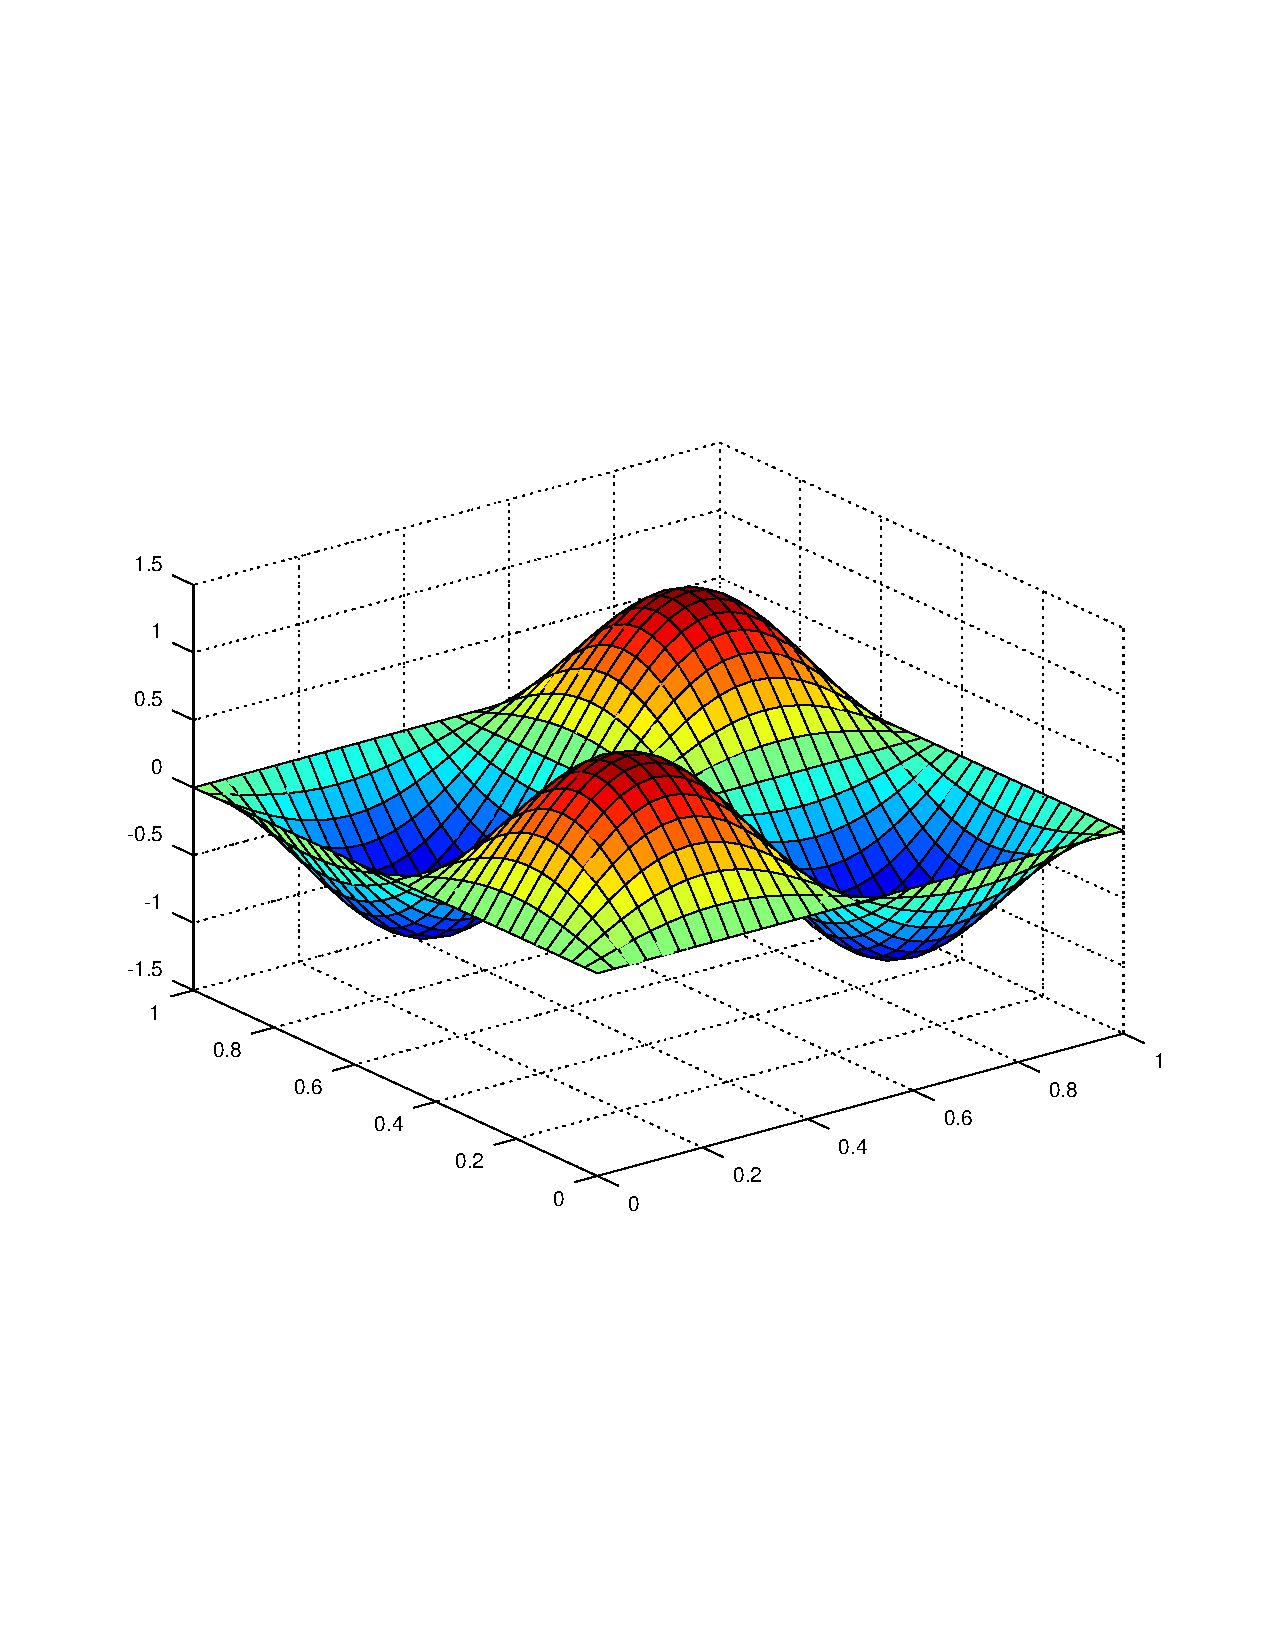
\includegraphics[height=40em]{a5l5}
		\end{center}
	\end{frame}
	\begin{frame}
		\frametitle{Aufgabe 5 -- Genauigkeit}
		Stellschrauben: $\varepsilon_{cg}, \varepsilon_{ILU}, \varepsilon_{GSV}$ \\
		\vspace{2em}
		Auswirkung auf den Fehler:
		\begin{center}
			\begin{tabular}{r|r|r|r|r}
				$\varepsilon_{cg}$ & $\varepsilon_{ILU}$ & $\varepsilon_{GSV}$ & Fehler $\epsilon_i$ & $\Delta\epsilon_i$ \\
				\hline
				$10^{-3}$ & $10^{-3}$ & $10^{-3}$ & $2,20\times10^{-4}$ & 0 \\
				$10^{-6}$ & $10^{-3}$ & $10^{-3}$ & $5,14\times10^{-5}$ & $-1,69\times10^{-4}$ \\
				$10^{-3}$ & $10^{-6}$ & $10^{-3}$ & $1,97\times10^{-4}$ & $-2,30\times10^{-5}$ \\
				$10^{-3}$ & $10^{-3}$ & $10^{-6}$ & $2,14\times10^{-4}$ & $-6,02\times10^{-7}$ \\
				$10^{-12}$ & $10^{-3}$ & $10^{-3}$ & $5,02\times10^{-5}$ & $-1,70\times10^{-4}$ \\
				$10^{-12}$ & $10^{-12}$ & $10^{-12}$ & $5,02\times10^{-5}$ & $-1,70\times10^{-4}$
			\end{tabular}
		\end{center}
	\vspace{2em}
	$\rightarrow$$\varepsilon_{cg}$ hat größte Relevant; naheliegend, da Rest Approximation
	\end{frame}
	\begin{frame}
		\frametitle{Aufgabe 5 -- Beschleuniger}
		Bisher: Alles, außer Berechnung von $Br$ (2$\times$GSV), auf CPU per OpenMP \\
		\vspace{2em}
		Wenig sinnvoll, da:
		\begin{enumerate}
			\item Overhead durch Datenaustausch
			\item Keine gleichzeitige Auslastung
			\item GPU vermutlich schneller in den CPU-Aufgaben (Vektoroperationen)
		\end{enumerate}
	\end{frame}
	\begin{frame}
		\frametitle{Aufgabe 5 -- Beschleunigung}
		\begin{center}
			\begin{tabular}{r|r|r}
			$l$ & $S_{CPU\rightarrow GPU_a}[s]$ & $S_{GPU_a\rightarrow GPU_c}[s]$ \\
			\hline
			7 & 0,929 & 1,06 \\
			8 & 0,284 & 1,14 \\
			9 & 0,0352 & 1,11
		\end{tabular}
		\end{center}
		Vorteil geringer als gedacht...\\
		$Br$ teuerster Berechnungsschritt
	\end{frame}
	\begin{frame}
		\frametitle{Aufgabe 5 -- Skalarprodukt auf der GPU}
		Möglich mittels \texttt{atomic}-Operationen, aber nicht optimal \\
		\vspace{2em}
		Bessere Lösung: \emph{Reduction} (wie auch in OpenMP)
		\begin{center}
			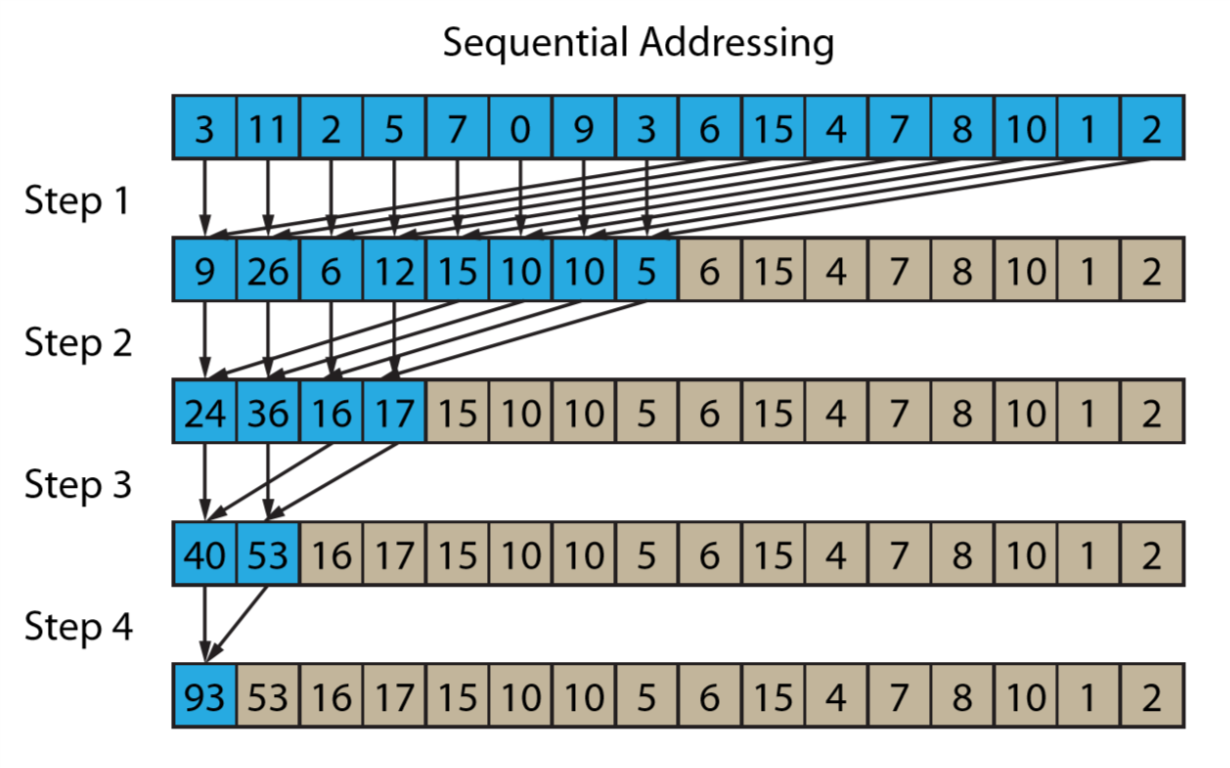
\includegraphics[height=14em]{reduction}
		\end{center}
	\end{frame}

	\section{Aufgabe 6}
	\subsection{Aufgabe 6}
	\begin{frame}
		\frametitle{Aufgabe 6 -- Lattice-Blotzmann-Methode}
		Maximale Größe des Gitters? \\
		Verfügbarer Speicherplatz auf der GPU $\approx2$ GB \\
		\vspace{2em}
		\pause
		Speicherbedarf für \texttt{rawdata1}, \texttt{rawdata2} und \texttt{u\_0}:
		\begin{equation*}
		\begin{split}
		M(\mathtt{rawdata1})&=M(\mathtt{rawdata2})\\
		&=max_x\cdot max_y\cdot max_z\cdot 19\cdot8\textsf{ Bytes} \\
		M(\mathtt{u\_0})&=max_x\cdot max_y\cdot 8\textsf{ Bytes}
		\end{split}
		\end{equation*}\\
		\vspace{2em}
		\pause
		Bedingung: $M(\mathtt{rawdata1})+M(\mathtt{rawdata2})+M(\mathtt{u\_0})\leq2.092.957.696$ \\
		Lösung: $max_x=max_y=max_z=190$
	\end{frame}
	\begin{frame}
		\frametitle{Aufgabe 6 -- Große Würfel}
		Würfel noch größer $\rightarrow$ passt nicht mehr in VRAM
	\end{frame}

	
	\section{Fazit}
	\subsection{Fazit}
	\begin{frame}
		\frametitle{Fazit}
		
		\LARGE
		\centering
		Mit \emph{CUDA} lässt es sich parallelisieren.
	\end{frame}

\end{document}